\documentclass[letterpaper,12pt]{exam}

\usepackage{ge05}
\usepackage{comment}
\usepackage{booktabs}
\usepackage[dvipdfm]{hyperref}
\urlstyle{rm}   % change fonts for url's (from Chad Jones)
\hypersetup{
    colorlinks=true,        % kills boxes
    allcolors=blue,
    pdfsubject={NYU Stern course GB 2303, Global Economy},
    pdfauthor={Dave Backus @ NYU},
    pdfstartview={FitH},
    pdfpagemode={UseNone},
%    pdfnewwindow=true,      % links in new window
%    linkcolor=blue,         % color of internal links
%    citecolor=blue,         % color of links to bibliography
%    filecolor=blue,         % color of file links
%    urlcolor=blue           % color of external links
% see:  http://www.tug.org/applications/hyperref/manual.html
}

\newcommand{\NX}{\mbox{\em NX\/}}
\newcommand{\POP}{\mbox{\em POP\/}}

\def\ClassName{The Global Economy}
\def\Category{Backus \& Cooley}
\def\HeadName{Midterm Examination}

\printanswers

\begin{document}
\parindent = 0.0in
\parskip = \bigskipamount
\thispagestyle{empty}%
\Head

\centerline{\large \bf \HeadName}%
%\centerline{March 9, 2005}
\centerline{Revised:  \today}

\bigskip
You have 90 minutes to complete this exam.  Please answer each
question in the space provided. You may consult one page of notes
and a calculator, but devices capable of wireless transmission are
prohibited.

I understand that the honor code applies: I will not lie, cheat,
or steal to gain an academic advantage, or tolerate those who do.

\begin{flushright}
\rule{4in}{0.5pt} \\ (Name and Signature)
\end{flushright}


%\begin{figure}[h]
%    \centering
%    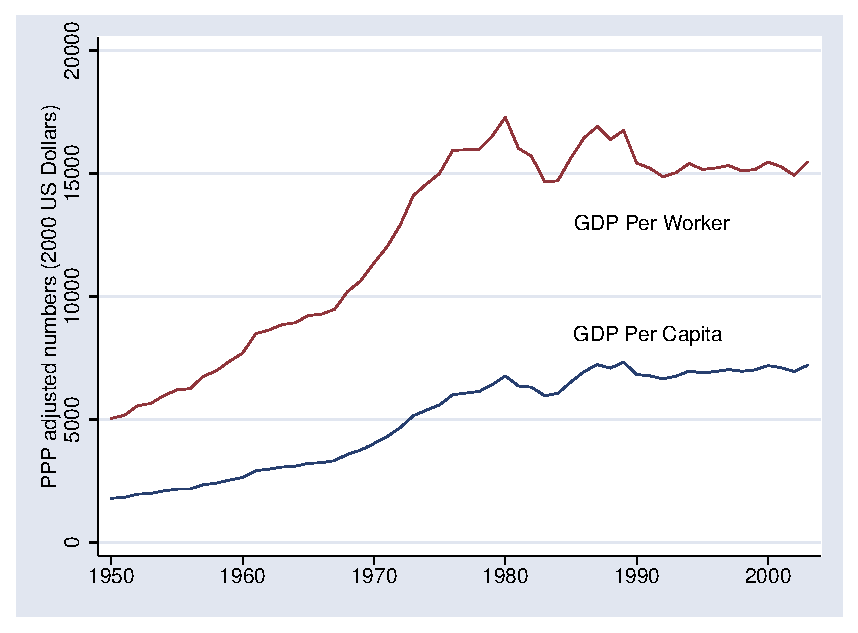
\includegraphics[scale=0.8]{pwtbramidterm07.eps}
%    \caption{GDP Per Capita and GDP Per Worker in Brazil.}
%    \label{fig:brazil}
%\end{figure}



\begin{questions}
% ======================================================================
\question 

%
\begin{parts}

\part 
(15~points)


\end{parts}


\begin{solution}
\begin{parts}
\part 
\end{parts}
\end{solution}

%\pagebreak \phantom{xx} \pagebreak \phantom{xx} \pagebreak
% ======================================================================
\question ...

\begin{parts}
\part
(10~points)

\end{parts}

\begin{solution}
\begin{parts}
\part
\end{parts}
\end{solution}

%\pagebreak %\phantom{xx} \pagebreak \phantom{xx} \pagebreak
% ======================================================================
\question {\it Miscellany.\/}
%
\begin{parts}
\part unemployment...  
\part 

\part (10~points)
\end{parts}

\begin{solution}
\begin{parts}

\part 
\end{parts}
\end{solution}

\end{questions}

%\pagebreak \phantom{xx} %\pagebreak \phantom{xx}

\vfill \centerline{\it \copyright \ \number\year \ NYU Stern
School of Business}

\end{document} 